\subsubsection{\cread}
%
A group of {\cread} gadgets read over a series of bit-bumps protruding into their row from the preceding row.
%
After a group of {\cread} gadgets read a bit pattern, a {\cread} gadget with a output length of $l$ produces a new bit pattern which it outputs to the {\prewarp} gadgets to begin the process of writing it in the row above it that encodes a copy or increment of the current digit.
%
If the input signal for a {\cread} gadget is {\tt copy}, it will always propagate a {\tt copy} signal.
%
However, if the input signal for a {\cread} gadget is {\tt increment}, the output will always depend on the bits of the digit that gets read.
%
First, if the value of the bits is less than $m - 1$, the digit can be incremented so the output of the {\cread} is the value read + 1, and a {\tt copy} signal is started.
%
Otherwise, the value of the bits is $m - 1$ so the digit is reset to 0, but the {\cread} gadget needs to check the two least signicant bits that it read to determine whether it should output a {\tt increment} or {\tt halt} signal.
%
There are 3 possible values for these bits, 00, 01, and 11.
%
If the bits are 00 or 01, an {\tt increment} signal will be output.
%
If the bits are 11, a {\tt halt} signal will be output, as these bits indicate this digit is the most significant digit in the most significant digit region.
%
By passing a {\tt halt} signal to the {\prewarp} gadget, this signal continues through the rest of the {\warpunit} gadgets and into a special {\cwrite} gadget, which will allow for the {\roofunit} to take over and complete the rectangle.
%
\begin{itemize}
    \item For each $i = 1,2,3$,
                   $j = 0,\ldots,l-2$,
                   $u \in \{0, 1\}^j$, and each
                   $\inc \in \{{\tt increment}, {\tt copy} \}$:
    \begin{itemize}
        \item Create
        $\begin{aligned}[t]
            \cread(& \left\langle {\tt CounterRead}, i, \lambda, \inc \right\rangle, \\
                   & \left\langle {\tt CounterRead}, i, 0,       \inc \right\rangle, \\
                   & \left\langle {\tt CounterRead}, i, 1,       \inc \right\rangle \;)
        \end{aligned}$\\ from the general gadget in Figure~\ref{fig:counter_read}.
    \end{itemize}
    %
    Note that 9 tiles are added for a single {\cread} gadget.
    %
    In this step,
    %
    \begin{align*}
        \sum_{j=0}^{l - 2} 9 \cdot 2 \cdot 3 \cdot 2^j &=    27 \left( 2^{l} - 2\right)\\
                                                       &=    27 \left( 2^{\ceil*{\log m} + 2} - 2 \right) \\
                                                       &=    27 \left(4 \cdot 2^{\ceil*{\log m}} - 2 \right) \\
                                                       &=    108 \left( 2^{\ceil*{\log m}} - \frac{1}{2} \right) \\
                                                       &\leq 108 \left(2 \cdot 2^{\log m} - \frac{1}{2} \right) \\
                                                       &=    108 \left(2m - \frac{1}{2} \right) \\
                                                       &=    216m - 81\\
                                                       &=    O(m) = O\left( \upperbound \right)\\
    \end{align*}
    %
    tiles were created in this step.
    %
\end{itemize}

\begin{itemize}
    \item For each $i = 1,2,3$ and each $u \in \{0, 1\}^{l-1}$:

    \begin{itemize}
        \item Create $\begin{aligned}[t]
            \cread(& \left\langle {\tt CounterRead}, i,  u, {\tt copy} \right\rangle,
                     \left\langle {\tt PreWarp},     i, 0u, {\tt copy} \right\rangle,
                     \left\langle {\tt PreWarp},     i, 1u, {\tt copy} \right\rangle \;)
        \end{aligned}$\\from the general gadget in Figure~\ref{fig:counter_read}.
    \end{itemize}


    Since the counter must only increment the current value if the result will be less than $m$,
    the \\{\cread} gadgets that have both an {\tt increment} signal and input size of $l - 2$ must
    first right shift the bits 2 spots, and then for each possible value after reading one more bit,
    check whether that value is less than $m - 1$. % counting in base-M implies that each digit must be less than M %.
    %
    Basically, if the next bit read is a 0, we check if the current value + 1 is less than $m$.
    %
    %
    %
    % If the counter is counting in base 8, (m is 8), then each digit has 3 (value) + 2 (indicator) bits.
    % The max digit value is "111"
    % Here we'd be on the last/most significant bit, so we've read "0100", and now let's pretend the next
    % bit is a "1", so the output would be "10100" IF this was a copy row.
    %
    % But we're incrementing, so focusing only on the digit value of "101"...
    %
    % Since the next bit is in the log(M) - 1's index, this means we must add 2^ log(M) - 1 to
    % "01" (the current value). We call this the final value of the digit.
    %
    % So adding 2^log2(M) - 1 to the final value, we get "101". Then, once we know the final value,
    % we check to see if the final value + 1 is less than M. If it is, the digit can be incremented
    % and we change the increment signal to a copy signal and pass along the final value + 1 as the next digit
    % to write, otherwise we output all zeroes and keep the increment signal.
    %
    If the next bit read is a 1, we check if current value + $2^{\log (m) - 1}$ + 1 is less than $m$.
    %
    For both cases, if the counter can increment the current value, then the {\cread} gadgets output the incremented value and a {\tt copy} signal to the {\prewarp} gadgets.
    %
    Otherwise, if the counter is unable to increment the value, it will output a signal in which the bits of the digit are all zeroes and the {\tt increment} signal is propagated to the next digit.
    %
    \begin{algorithm}[H]
        \caption{Incrementing and halting\label{asda}}
        \begin{algorithmic}[1]
            \Function{ReadMostSignicantBit}{ }
                \State $guess0 \gets 0u >> 2$.
                \State $guess1 \gets 1u >> 2$.
                \If{$convertToDecimal(guess0) + 1 \leq m - 1$}
                    \State $out0 \gets \left\langle {\tt PreWarp}, i, convertToBinary(convertToDecimal(guess0) + 1) + u[1] + [0], {\tt copy} \right\rangle$.
                \Else
                    \If{$u$ ends with ``11"}
                        \State $out0 \gets \left\langle {\tt PreWarp}, i, repeat(``0", m) + 11, {\tt halt} \right\rangle$.
                    \Else
                        \State $out0 \gets \left\langle {\tt PreWarp}, i, repeat(``0", m) + u[1] + u[0], {\tt increment} \right\rangle$.
                    \EndIf
                \EndIf
                \If{$convertToDecimal(guess1) + 1 \leq m - 1$}
                    \State $out1 \gets \left\langle {\tt PreWarp}, i, convertToBinary(convertToDecimal(guess1) + 1) + u[1] + [0], {\tt copy} \right\rangle$.
                \Else
                    \If{$u$ ends with ``11"}
                        \State $out1 \gets \left\langle {\tt PreWarp}, i, repeat(``0", m) + 11, {\tt halt} \right\rangle$.
                    \Else
                        \State $out1 \gets \left\langle {\tt PreWarp}, i, repeat(``0", m) + u[1] + u[0], {\tt increment} \right\rangle$.
                    \EndIf
                \EndIf
            \EndFunction
        \end{algorithmic}
    \end{algorithm}

    \begin{itemize}
        \item
        Create $\begin{aligned}[t]
                   \cread(& \left\langle {\tt CounterRead}, i, u, {\tt increment} \right\rangle, out0, out1 \;)
               \end{aligned}$\\from the general gadget in Figure~\ref{fig:counter_read}.
    \end{itemize}
    %
    Note $\{0, 1 \}^{l-1} =$ $\{0, 1\}^{\ceil*{\log m} + 1}$, so
    %
    $\left| {\{0, 1\}^{\ceil*{\log m} + 1}} \right| =$
    %
    $2^{\ceil*{\log m}} + 2^1 \leq$
    %
    $4 \cdot 2^{\log m} =$
    %
    $4m$.
    %
    So in this step $O\left(m \right) = O\left( \upperbound \right)$ tiles were created.
    %

\end{itemize}

\begin{figure}[H]
    \centering
    \subcaptionbox{
        {\tt Counter\_Read\_0}
        \label{fig:counter_read_0}
    }{\makebox[0.24\textwidth][c]{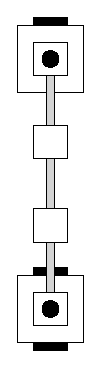
\includegraphics[width=0.33in]{counter_read_0}}}%
    ~
    \subcaptionbox{
        {\tt Counter\_Read\_1}
        \label{fig:counter_read_1}
    }{\makebox[0.24\textwidth][c]{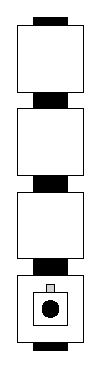
\includegraphics[width=0.33in]{counter_read_1}}}%
    ~
    \subcaptionbox{
        Digit 1 - general\\ overview.
        \label{fig:counter_read_1_op}
    }{\makebox[0.24\textwidth][c]{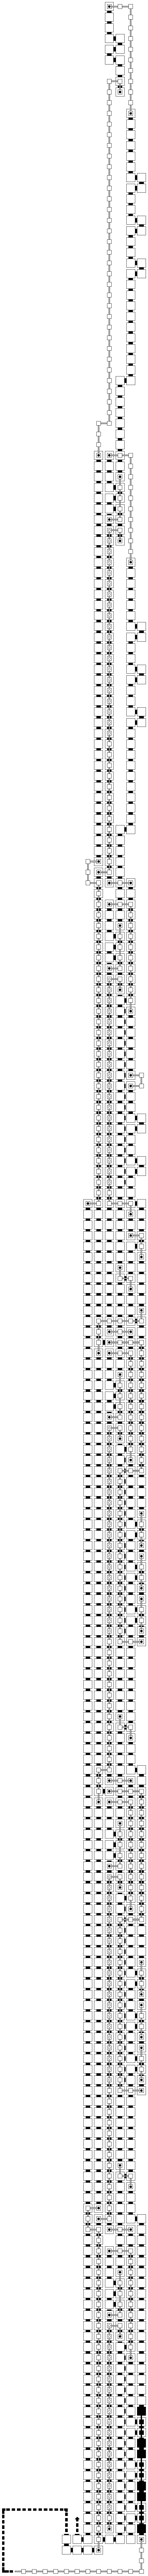
\includegraphics[width=0.45in]{overviews/general/counter_read_1_op}}}%
    ~
    \subcaptionbox{
        Digit 2 - general\\ overview.
        \label{fig:counter_read_2_op}
    }{\makebox[0.24\textwidth][c]{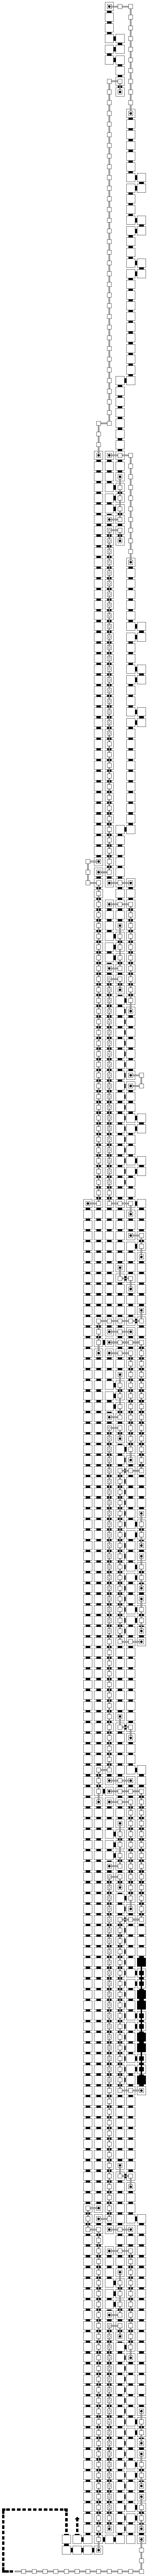
\includegraphics[width=0.45in]{overviews/general/counter_read_2_op}}}%
    ~
\end{figure}
\begin{figure}[H]\ContinuedFloat
    \centering
    \subcaptionbox{
        Digit 3 - general\\ overview.
        \label{fig:counter_read_3_op}
    }{\makebox[0.24\textwidth][c]{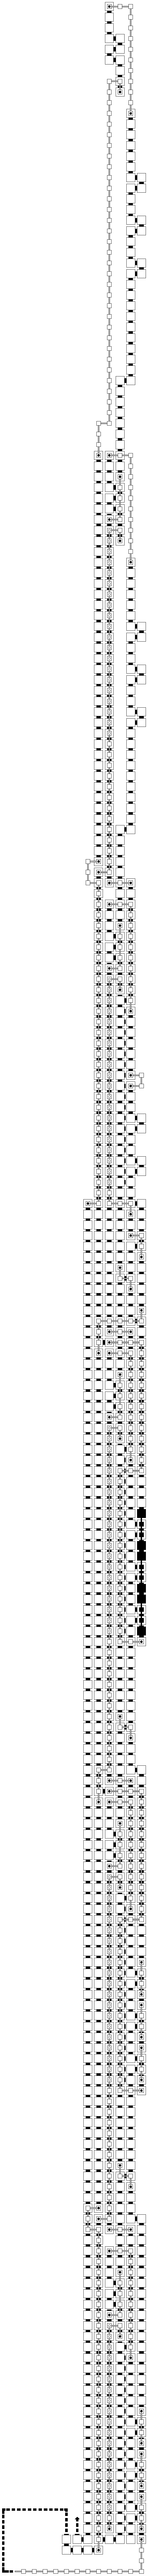
\includegraphics[width=0.45in]{overviews/general/counter_read_3_op}}}%
    ~
    \subcaptionbox{
        Digit 1 - case 1 overview.
        \label{fig:counter_read_1_op_msr_msd}
    }{\makebox[0.24\textwidth][c]{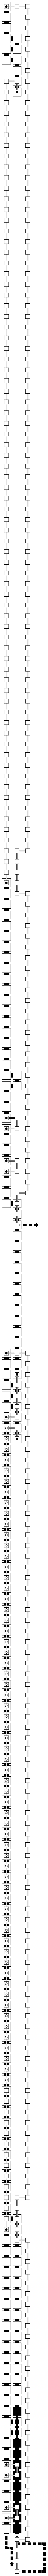
\includegraphics[width=0.45in]{overviews/case1/counter_read_1_op_msr_msd}}}%
    ~
    \subcaptionbox{
        Digit 1 - case 2 overview.
        \label{fig:counter_read_1_op_msr}
    }{\makebox[0.24\textwidth][c]{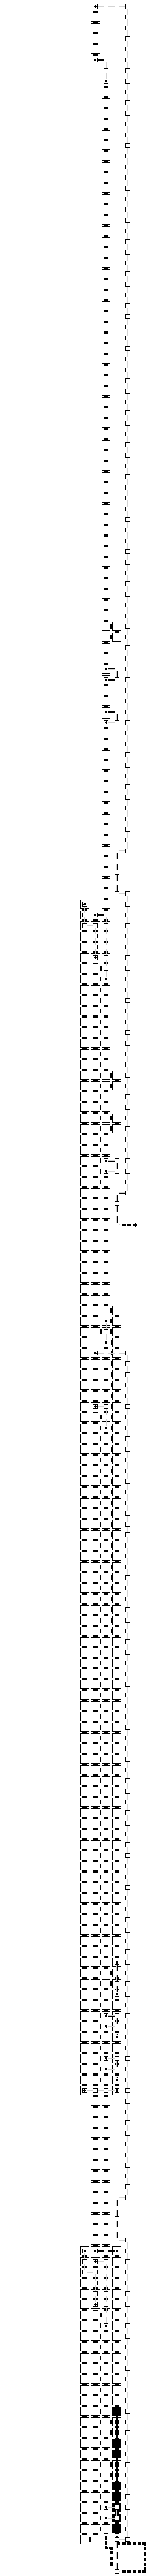
\includegraphics[width=0.45in]{overviews/case2/counter_read_1_op_msr}}}%
    ~
    \subcaptionbox{
        Digit 2 - case 2 overview.
        \label{fig:counter_read_2_op_msr_msd}
    }{\makebox[0.24\textwidth][c]{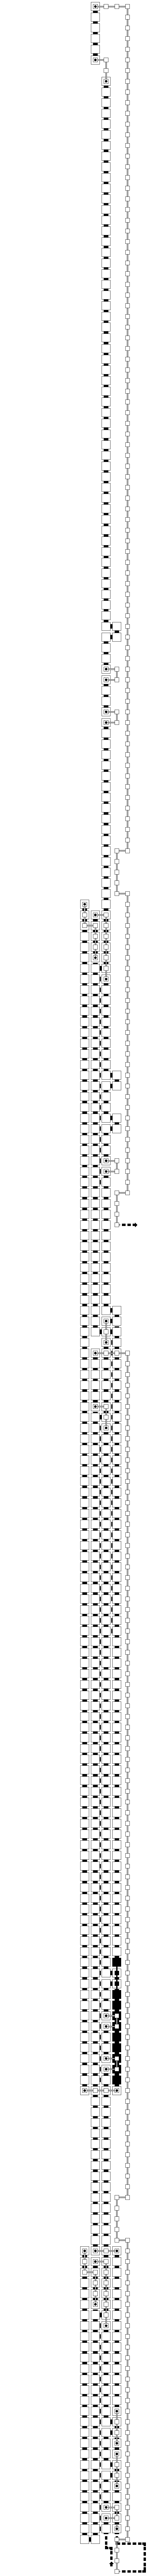
\includegraphics[width=0.45in]{overviews/case2/counter_read_2_op_msr_msd}}}%
    ~
\end{figure}
\begin{figure}[H]\ContinuedFloat
    \centering
    \subcaptionbox{
        Digit 3 - case 3\\ overview.
        \label{fig:counter_read_3_op_msr_msd}
    }{\makebox[0.24\textwidth][c]{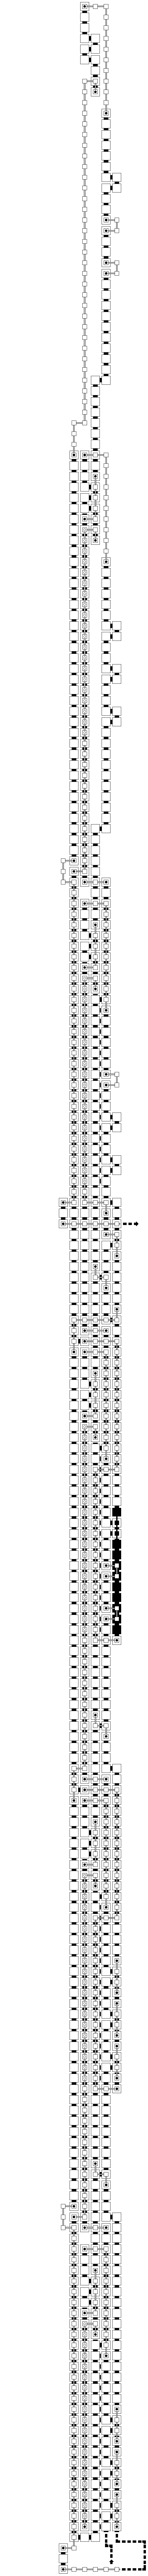
\includegraphics[width=0.45in]{overviews/case3/counter_read_3_op_msr_msd}}}%
    ~
    \caption{\label{fig:counter_read} The {\cread} gadgets.}
\end{figure}